% Afficher des recommendations concernant la syntaxe.
\RequirePackage[orthodox,l2tabu]{nag}
\RequirePackage{luatex85}
% Paramètres du document.
\documentclass[%
a6paper%                       Taille de page.
,11pt%                         Taille de police.
,DIV=auto%                       Plus grand => des marges plus petites.
,titlepage=on%                 Faut-il une page de titre ?
,headings=optiontoheadandtoc%  Effet des paramètres optionnels de section.
,headings=small%
,parskip=false%
,openany%
]{scrbook}
\renewcommand*\partheademptypage{\thispagestyle{empty}}
\newcounter{facteur}\setcounter{facteur}{17}%%%%%%%%%%%%%% Paramètre pour la taille globale des partitions. par défaut~: 17
%\usepackage{geometry}
\usepackage{gredoc,mudoc,lyluatex}
\usepackage{pdfpages,transparent,array,ltablex}

%%%%%%%%%%%%%%%%%%%%%%% Paramètres variables %%%%%%%%%%%%%%%%%%%%%%%%%%%%%%%%%%%%%%%%%%%%%%%%%%
%%% Taille des partitions grégoriennes.                                                      %%
%\grechangedim{overhepisemalowshift}{.7mm}{scalable}
%\grechangedim{hepisemamiddleshift}{1.4mm}{scalable}
%\grechangedim{overhepisemahighshift}{2.1mm}{scalable}
%\grechangedim{vepisemahighshift}{2.1mm}{scalable}
%\grechangestafflinethickness{50} %%% epaisseur des lignes
\grechangestaffsize{\value{facteur}}%%%%% 
%%%%%%%%%%%%%%%%%%%%%%%%%%%%%%%%%%%%%%%%%%%%%%%%%%%%%%%%%%%%%%%%%%%%%%%%%%%%%%%%%%%%%%%%%%%%%%%
% Par souci de clarté, la définition des commandes est reportée dans un document annexe.

%\addtolength{\voffset}{2mm}\addtolength{\headsep}{-2mm}
%\setlength{\extrarowheight}{2mm}

\addto\captionsfrench{%
  \renewcommand{\indexname}{Index des chants}%
}

\pdfcompresslevel=9

\newcommand{\lieu}[1]{\hfill\linebreak[3]\hspace*{\stretch{1}}\nolinebreak\mbox{\emph{(#1)}}}


\newcommand{\schola}[1]{}\newcommand{\foule}[1]{#1}
\providecommand{\dest}{foule}
\newcommand{\imagecentre}[2]{
\begin{center} \includegraphics[height=#1]{img/#2} \end{center}}

%\newcommand{\bgimage}[1]{%
%\raisebox{-.45\paperheight}[0pt][0pt]{%
%  \transparent{0.3}%
%  \includegraphics[width=.7\paperwidth,height=.7\paperheight,keepaspectratio=true]{img/#1}%
%  }%
%}

\def\arraystretch{1.2}

\newcommand{\reponsegras}[2]{
\versio{\textbf{#1}}{{#2}}}

\newcommand{\ligne}[2]{
\begin{center}
\greseparator{#1}{#2}
\end{center}}

\title{Livret du Pèlerin de Fontpeyrine}
\date{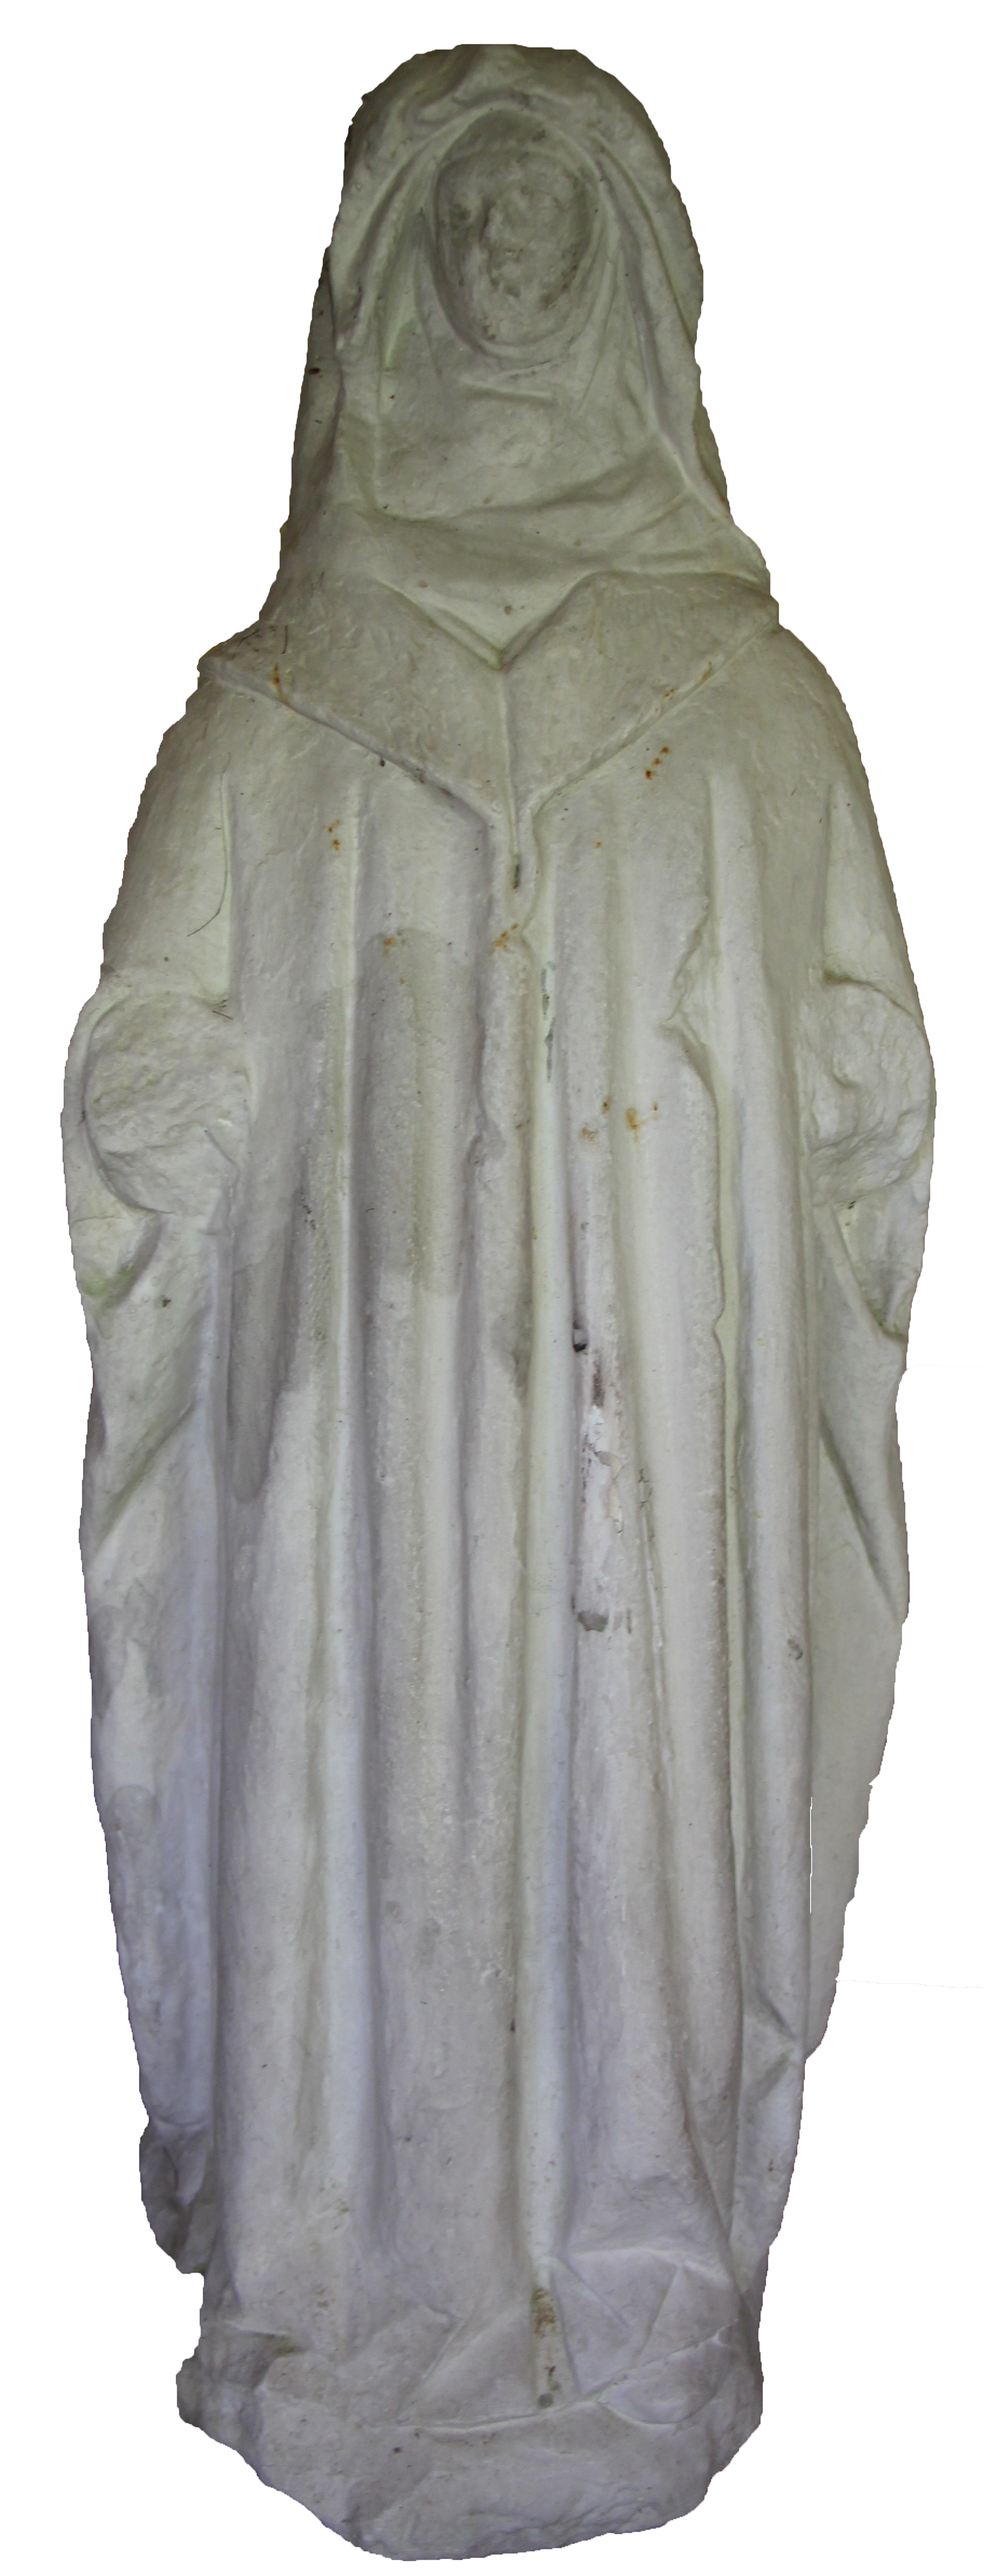
\includegraphics[width=.3\textwidth]{img/Fontpeyrine-Vierge-source.png}}

\let\oldaddchap\addchap
\def\addchap#1{\oldaddchap{#1}\markright{Livret du Pèlerin de Fontpeyrine}}

\def\blindsection#1{\markright{#1}\addcontentsline{toc}{section}{#1}}
%%%%%%%%%%%%%%%%%%%%%%%%%%%%%%%%%%%%%%%%%%%%%%%%%%%%%%%%%%%%%%%%%%%%%%%%%%%%%%%%
%%%%%%%%%%%%%%%%%%%%%% Début du document %%%%%%%%%%%%%%%%%%%%%%%%%%%%%%%%%%%%%%%
%%%%%%%%%%%%%%%%%%%%%%%%%%%%%%%%%%%%%%%%%%%%%%%%%%%%%%%%%%%%%%%%%%%%%%%%%%%%%%%%
\begin{document}
\maketitle

\addchap{Prière à Notre-Dame de Fontpeyrine}
{\centering {\textit{\Large{Notre-Dame de Fontpeyrine,\vfill
qui depuis des siècles accordez de nombreuses faveurs\vfill
à ceux qui ont recours à votre puissante intercession,\vfill
obtenez, nous vous en supplions,\vfill
à nous vos humbles serviteurs, \vfill
en souvenir de votre bienheureuse Nativité,\vfill
ce complément de grâce\vfill
que nous implorons à genoux devant vous.\vfill
Nous l’attendons avec confiance,\vfill
malgré notre indignité, ô Mère du Sauveur,\vfill
de votre maternelle bonté\vfill
et de votre bienveillante protection.\vfill
Ainsi soit-il.\vfill
Notre-Dame de Fontpeyrine, priez pour nous (trois fois).}}}}
\clearpage

\addchap{Cantiques}
%\blindsection{Cantiques}
\section{Vierge de Fontpeyrine}
\lilypondfile[staffsize=15]{ly/ViergeDeFontpeyrine/ViergeDeFontpeyrine.ly}
\chanson[position=2col,numero=2,premiercouplet=2,refrain=non]{ly/ViergeDeFontpeyrine/ViergeDeFontpeyrine}
%\lilypondfile[staffsize=15]{ly/ViergeDeFontpeyrine/ViergeDeFontpeyrine-dernier.ly}

\section{C'est le Périgord}
\lilypondfile[staffsize=15]{ly/CestLePerigord/CestLePerigord.ly}
\chanson[position=2col,numero=2,premiercouplet=2,refrain=non]{ly/CestLePerigord/CestLePerigord}

\section{Notre-Dame du Périgord}
\lilypondfile[staffsize=15]{ly/NotreDameDuPerigord/NotreDameDuPerigord.ly}
\chanson[position=2col,numero=2,premiercouplet=2,refrain=non]{ly/NotreDameDuPerigord/NotreDameDuPerigord}

\section{Les saints et les anges}
\chanson[position=2col,numero=1]{ly/AveMariaDeLourdes/LesSaintsEtLesAnges}


\section{J'irai la voir un jour}
\chanson[position=2col,numero=1]{ly/JIraiLaVoirUnJour/JIraiLaVoirUnJour}

\section{Vierge sainte}
\chanson[position=2col,numero=1]{ly/ViergeSainte/ViergeSainte}

\section{Laudate Mariam}
\chanson[position=2col,numero=1]{ly/LaudateMariam/LaudateMariam}

\section{Ave Maris Stella}
\chanson[position=2col,numero=1]{ly/AveMarisStella/AveMarisStella}

\section{Reine de France}
\chanson[numero=1]{ly/ReineDeFrance/ReineDeFrance}

\section{Je mets ma confiance}
\chanson[position=2col,numero=1]{ly/JeMetsMaConfiance/JeMetsMaConfiance}

\section{Chez nous, soyez Reine}
\chanson[position=2col,numero=1]{ly/ChezNousSoyezReine/ChezNousSoyezReine}

\needspace{8\baselineskip}
\section{Tandis que le monde proclame}
\chanson[position=2col,numero=1]{ly/ParleCommandeRegne/ParleCommandeRegne}

\section{Je suis chrétien}
\chanson[position=2col,numero=1]{ly/JeSuisChretien/JeSuisChretien}

\section{Nous voulons Dieu}
\chanson[position=2col,numero=1]{ly/NousVoulonsDieu/NousVoulonsDieu}

\section{Litanies de la très sainte Vierge}
\begin{litaniae}
\invocatio{Kýrie, eléison.}{Seigneur, ayez pitié de nous.}
\invocatio{Christe, eléison.}{Jésus-Christ, ayez pitié de nous.}
\invocatio{Kýrie, eléison.}{Seigneur, ayez pitié de nous.}
\invocatio{Christe, audi nos.}{Jésus-Christ, écoutez-nous.}
\invocatio{Christe, exáudi nos.}{Jésus-Christ, exaucez-nous.}
\rinvocatio{Pater de cælis, Deus,}{Père céleste qui êtes Dieu,}{miserére nobis.}{ayez pitié de nous.}
\invocatio{Fili, Redémptor mundi, Deus,}{Fils Rédempteur du monde, qui êtes Dieu,}
\invocatio{Spíritus Sancte, Deus,}{Esprit Saint, qui êtes Dieu,}
\invocatio{Sancta Trínitas, unus Deus,}{Trinité Sainte, qui êtes un seul Dieu,}
\rinvocatio{Sancta María}{Sainte Marie}{ora pro nobis.}{priez pour nous.}
\invocatio{Sancta Dei Genitrix,}{Sainte Mère de Dieu,}
\invocatio{Sancta Virgo virginum,}{Sainte Vierge des vierges,}
\invocatio{Mater Christi,}{Mère du Christ,}
\invocatio{Mater Ecclesiae,}{Mère de la Sainte Eglise,}
\invocatio{Mater divinae gratiae,}{Mère de la divine grâce,}
\invocatio{Mater purissima,}{Mère très pure,}
\invocatio{Mater castissima,}{Mère très chaste,}
\invocatio{Mater inviolata,}{Mère toujours Vierge,}
\invocatio{Mater intemerata,}{Mère sans tache,}
\invocatio{Mater amabilis,}{Mère aimable,}
\invocatio{Mater admirabilis,}{Mère admirable,}
\invocatio{Mater boni consilii,}{Mère du bon conseil,}
\invocatio{Mater Creatoris,}{Mère du Créateur,}
\invocatio{Mater Salvatoris,}{Mère du Sauveur,}
\invocatio{Virgo prudentissima,}{Vierge très prudente,}
\invocatio{Virgo veneranda,}{Vierge vénérable,}
\invocatio{Virgo praedicanda,}{Vierge digne de louange,}
\invocatio{Virgo potens,}{Vierge puissante,}
\invocatio{Virgo clemens,}{Vierge clémente,}
\invocatio{Virgo fidelis,}{Vierge fidèle,}
\invocatio{Speculum justitiae,}{Miroir de justice,}
\invocatio{Sedes sapientiae,}{Trône de la sagesse,}
\invocatio{Causa nostrae laetiae,}{Cause de notre joie,}
\invocatio{Vas spirituale,}{Vase spirituel,}
\invocatio{Vas honorabile,}{Vase d'honneur,}
\invocatio{Vas insigne devotionis,}{Vase insigne de dévotion,}
\invocatio{Rosa mystica,}{Rose mystique,}
\invocatio{Turris Davidica,}{Tour de David,}
\invocatio{Turris ebumea,}{Tour d'ivoire,}
\invocatio{Domus aurea,}{Maison d'or,}
\invocatio{Fœderis arca,}{Arche d'alliance,}
\invocatio{Janua Caeli,}{Porte du ciel,}
\invocatio{Stella matutina,}{Étoile du matin,}
\invocatio{Salus infirmorum,}{Salut des infirmes,}
\invocatio{Refugium peccatorum,}{Refuge des pécheurs,}
\invocatio{Consolatrix afflictonim,}{Consolatrice des affligés,}
\invocatio{Auxilium Christianorum,}{Secours des chrétiens,}
\invocatio{Regina Angelorum,}{Reine des Anges,}
\invocatio{Regina Patriarcharum,}{Reine des Patriarches,}
\invocatio{Regina Prophetarum,}{Reine des Prophètes.}
\invocatio{Regina Apostolorum,}{Reine des Apôtres,}
\invocatio{Regina Martyrum,}{Reine des Martyrs,}
\invocatio{Regina Confessorum,}{Reine des Confesseurs,}
\invocatio{Regina Virginum,}{Reine des Vierges,}
\invocatio{Regina Sanctorum omnium,}{Reine de tous les Saints}
\invocatio{Regina sine labe originali concepta}{Reine conçue sans le péché originel,}
\invocatio{Regina in caelum assumpta,}{Reine élevée aux Cieux,}
\invocatio{Regina sacratissimi Rosarii,}{Reine du très saint Rosaire,}
\invocatio{Regina pacis,}{Reine de la paix,}
\rinvocatio{Agnus Dei, qui tollis peccáta mundi,}{Agneau de Dieu, qui effacez les péchés du monde,}%
{parce nobis, Dómine.}{pardonnez-nous, Seigneur.}
\rinvocatio{Agnus Dei, qui tollis peccáta mundi,}{Agneau de Dieu, qui effacez les péchés du monde,}%
{exáudi nos, Dómine.}{exaucez-nous, Seigneur.}
\rinvocatio{Agnus Dei, qui tollis peccáta mundi,}{Agneau de Dieu, qui effacez les péchés du monde,}%
{miserére nobis.}{ayez pitié de nous.}
\end{litaniae}
\versio{\vb. Ora pro nobis, sancta Dei Génetrix,}{\vb. Priez pour nous sainte Mère de Dieu,}
\reponsegras{\rb. Ut digni efficiámur promissiónibus Christi.}{\vb. Afin que nous soyons dignes des promesses du Christ.}
\versio{\centering{Orémus}

Concéde nos fámulos tuos, quǽsumus, Dómine Deus, perpétua mentis et córporis sanitáte gaudére\* : et, gloriósa beátæ Maríæ semper Vírginis intercessióne\+, a præsénti liberári tristítia et ætérna pérfrui lætítia. Per Christum Dóminum nostrum.\mbox{\textbf{℟. Amen.}}}
{\centering{Prions.}

Seigneur, daignez nous accorder, à nous vos serviteurs, de jouir toujours de la santé de l'âme et du corps; et par la glorieuse intercession de la bienheureuse Marie toujours Vierge, délivrez-nous des tristesses de la vie présente, et donnez-nous d'avoir part aux joies éternelles. Par Jésus-Christ Notre Seigneur.\mbox{\textbf{℟. Ainsi soit-il.}}}

%%%%%%%%%%%%%%%%%%%%%%%%%%%%%%%%%%%%%%%%%%%%%%%%%%%%%%%%%%%%%%%%%%%%%%%%%%%%%%%%

\end{document}